\documentclass[letterpaper,11pt]{article}

\usepackage{amsmath}
\usepackage[hmargin=1.25in,vmargin=1in]{geometry}
\usepackage{graphicx}
\usepackage{hyperref}
\usepackage{listings}
\usepackage{lmodern}
\usepackage{microtype}
\usepackage{minted}

\DeclareMathOperator*{\argmin}{arg\,min}

\author{Philip Pham}
\date{\today}
\title{CSE 547 - Assignment 1}

\begin{document}
\maketitle

\section*{Problem 0}

\begin{description}
\item[List of collaborators:] I have not collaborated with anyone.
\item[List of acknowledgements:] None.
\item[Certify that you have read the instructions:] Yes.
\item[Terms and Conditions to use the dataset:] I accept the terms and conditions to use the COCO dataset.  
\end{description}

\section*{Problem 1}

Read the course website, up until ``Lecture Notes and Readings'', so
that you understand the course policies on grading, late policies,
projects, requirements to pass etc. Write ``I have read and understood
these policies'' to certify this. If you have questions, please contact
the instructors.

\subsection*{Solution}

I have read and understood these policies.

\section*{Problem 2}

Consider the function from class (and the notes):
\begin{equation}
  f\left(w_1,w_2\right) = \left[\sin\left(2\pi\frac{w_1}{w_2}\right) + 3\frac{w_1}{w_2} - \exp\left(2w_2\right)\right]\left[3\frac{w_1}{w_2} - \exp\left(2w_2\right)\right].
\end{equation}

Suppose our program for this function uses the following evaluation trace:

\begin{description}
\item[input:] $z_0 = \left(w_1,w_2\right)$
  \begin{enumerate}
  \item $z_1 = w_1/w_2$
  \item $z_2 = \sin\left(2\pi z_1\right)$
  \item $z_3 = \exp\left(2w_2\right)$
  \item $z_4 = 3z_1 - z_3$
  \item $z_5 = z_2 + z_4$
  \item $z_6 = z_4z_5$
  \end{enumerate}
\item[return:] $z_6$
\end{description}

\subsection*{The forward mode of AD}

The forward mode for auto-differentiation is a conceptually simpler way to compute the derivative. Let us examine the forward mode to compute the derivative of one variable, $\frac{df}{dw_1}$. In the forward mode, we sequentially compute both $z_t$ and its derviative $\frac{dz_t}{dw_1}$ using the previous variables $z_1,\ldots,z_{t-1}$ and the previous derivatives $\frac{dz_1}{dw_1},\ldots,\frac{dz_{t-1}}{dw_1}$.

Explicitly write out the forward mode in our example.

\subsubsection*{Solution}

\begin{align*}
  \frac{df}{dw_1} = \frac{dz_6}{dw_1}
  &= \frac{\partial z_6}{\partial z_4}\frac{dz_4}{dw_1} +
    \frac{\partial z_6}{\partial z_5}\frac{dz_5}{dw_1} \\
  &= \frac{\partial z_6}{\partial z_5}\left(
    \frac{\partial{z_4}}{\partial{z_1}}\frac{dz_1}{dw_1} +
    \frac{\partial{z_4}}{\partial{z_3}}\frac{dz_3}{dw_1}
    \right) +
    \frac{\partial z_6}{\partial z_5}\left(
    \frac{\partial{z_5}}{\partial{z_2}}\frac{dz_2}{dw_1} +
    \frac{\partial{z_5}}{\partial{z_4}}\frac{dz_4}{dw_1}
    \right) \\
  &= \frac{\partial z_6}{\partial z_5}\left(
    \frac{\partial{z_4}}{\partial{z_1}}\frac{dz_1}{dw_1} +
    \frac{\partial{z_4}}{\partial{z_3}}\frac{dz_3}{dw_1}
    \right) +
    \frac{\partial z_6}{\partial z_5}\left(
    \frac{\partial{z_5}}{\partial{z_2}}\frac{dz_2}{dw_1} +
    \frac{\partial{z_5}}{\partial{z_4}}\left(
    \frac{\partial{z_4}}{\partial{z_1}}\frac{dz_1}{dw_1} +
    \frac{\partial{z_4}}{\partial{z_3}}\frac{dz_3}{dw_1}
    \right)
    \right)
\end{align*}

Suppose we want to calculate $\frac{df}{dw_1}(u,v)$.

\begin{enumerate}
\item Fix $w_1 = u$ and $w_2 = v$.
\item Compute $z_1 = u/v$ and $\frac{dz_1}{w_1} = 1/v$.
\item Compute $z_2 = \sin\left(2\pi z_1\right)$ and $\frac{dz_2}{dw_1} = \frac{\partial z_2}{\partial z_1}\frac{dz_1}{w_1} = 2\pi\cos\left(2\pi z_1\right)\frac{dz_1}{w_1}$.
\item Compute $z_3 = \exp\left(2v\right)$ and $\frac{dz_3}{dw_1} = 0$.
\item Compute $z_4 = 3z_1 - z_3$ and
\begin{align*}
  \frac{dz_4}{dw_1}
  &= \frac{\partial z_4}{\partial z_1}\frac{dz_1}{dw_1} + \frac{\partial z_4}{\partial z_3}\frac{dz_3}{dw_1} = 3\frac{dz_1}{dw_1} - \frac{dz_3}{dw_1}.
\end{align*}
\item Compute
  $z_5 = z_2 + z_4$ and
  \begin{align*}
  \frac{dz_5}{dw_1}
    &= \frac{\partial z_5}{\partial z_2}\frac{dz_2}{dw_1} + \frac{\partial z_5}{\partial z_4}\frac{dz_4}{dw_1} \\
    &= \frac{dz_2}{dw_1} + \frac{dz_4}{dw_1}.
  \end{align*}
\item Compute $z_6 = z_4z_5$ and
  \begin{align*}
    \frac{dz_6}{dw_1} = \frac{\partial z_6}{\partial z_4}\frac{dz_4}{dw_1} +
    \frac{\partial z_6}{\partial z_5}\frac{dz_5}{dw_1} = z_5\frac{dz_4}{dw_1} +
    z_4\frac{dz_5}{dw_1}.
  \end{align*}
\end{enumerate}

\subsection*{The reverse mode of AD}

Now let use consider the reverse mode to compute the derivative
$\frac{df}{dw}$, which is a two-dimensional vector.

Explicitly write out the reverse mode in our example.

\subsubsection*{Solution}

\section*{Problem 4: PyTorch can give us some crazy answers}

Now you will construct an example in which PyTorch provides derivatives that
make no sense. The issue is in understanding when it is ok and when it is not ok
to use dynamic computation graphs. You are going to find a way code up the same
function in two different ways so that PyTorch will return different derivatives
at the same point. The purpose of this exercise is to better understand how
dynamic computation graphs work and to understand what you are doing when you
using various AD softwares.

\subsection*{Two Identical Non-differentiable Functions with Different ``Derivatives''}

\begin{enumerate}
\item Define \emph{and} plot a one dimensional, real valued function
  which is not continuous.
  
  \subsubsection*{Solution}
  Consider the function
  \begin{equation}
    f(x) = \begin{cases}
      2x, - 1& x < 0; \\
      0, & x = 0; \\
      2x + 1, & x > 0.
    \end{cases}
    \label{eqn:problem4}
  \end{equation}

  It is implemented in Listings \ref{lst:f} and \ref{lst:g} and plotted in
  Figure \ref{fig:problem4}.

  \begin{figure}[h]
    \centering
    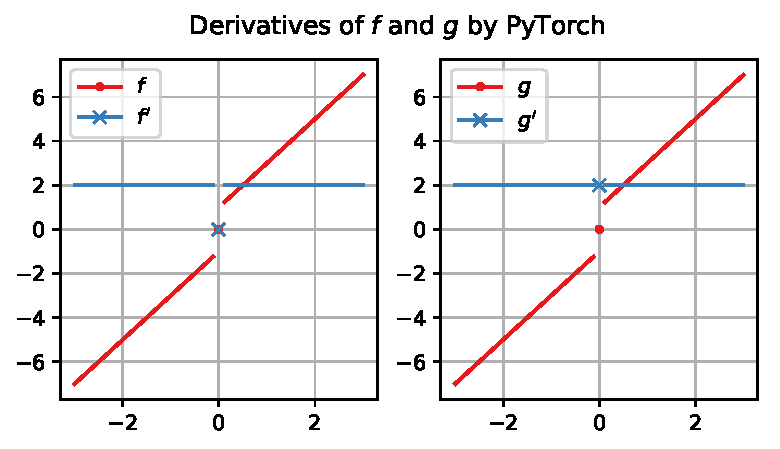
\includegraphics{problem4/problem4.pdf}
    \caption{The functions from Listings \ref{lst:f} and \ref{lst:g} are plotted
      along with their PyTorch-computed derivatives.}
    \label{fig:problem4}
  \end{figure}
\item Now write out your function in PyTorch. You should be able to
  define this function so that PyTorch returns a derivative of $0$ at
  some point $x_0$.
  \subsubsection*{Solution}
  Equation \ref{eqn:problem4} is implemented as $f$ in Listing
  \ref{lst:f}. In Figure \ref{fig:problem4}, you can see that PyTorch
  calculates the derivative as $0$ at $x_0 = 0$ (left plot, blue
  \texttt{x}).
  
  \begin{listing}
\begin{minted}{python}
def f(x: Variable) -> Variable:
    assert x.requires_grad
    return (2*x*torch.sign(x) + 1)*torch.sign(x)
\end{minted}
  \caption{Equation \ref{eqn:problem4} defined with the sign function factored out.}
\label{lst:f}
\end{listing}

\item Now find another way to write out your function in PyTorch; do
  this so that it is exactly the same function. Do this in a way so
  that PyTorch now returns a derivative of $2$ at exactly the same
  point $x_0$ that you obtained a derivative of $0$ in the previous
  question.
  \subsubsection*{Solution}
  Equation \ref{eqn:problem4} is implemented as $g$ in Listing
  \ref{lst:g}. In Figure \ref{fig:problem4}, you can see that PyTorch
  calculates the derivative as $2$ at $x_0 = 0$ (right plot, blue
  \texttt{x}).
  
\begin{listing}
\begin{minted}{python}
def g(x: Variable) -> Variable:
    def g1d(x: Variable) -> Variable:
        if x.data[0] > 0:
            return 2*x + 1
        elif x.data[0] < 0:
            return 2*x - 1
        else:
            return 2*x

    if x.dim() == 0:
        return 1*x    
    if x.size() == torch.Size([1]):
        return g1d(x)

    return torch.stack([g(sub_x) for sub_x in x])
\end{minted}
  \caption{Equation \ref{eqn:problem4} defined element-wise by recursing into the tensor.}
\label{lst:g}
\end{listing}
\item There is a no sane definition of the derivative for your
  function. Yet, you should not only found a way to get PyTorch to
  provide a derivative, you should have also found a way to give you
  two \emph{different} derivatives at exactly the same point (on the same
  function). What went wrong?

  \subsubsection*{Solution}

  PyTorch is just keeping track of the operations and does a pointwise
  calculation. It's not paying attention to any local behvaior like
  continuity. In Listing \ref{lst:g}, by changing the \texttt{else}
  arm, we can have it return any arbitrary number for the
  derivative. For instance, having it return \texttt{-3*x} would have
  PyTorch calculating the derivative as $-3$ at $x_0 = 0$.
\end{enumerate}

\subsection*{Extra Credit: Differentiable Functions with Different ``Derivatives''}

Provide a differentiable function, where you can code it up in PyTorch
in two different ways and where you can get two different derivatives
at the same point $x_0$.

\subsubsection*{Solution}

We can reuse the same idea. PyTorch doesn't correctly compute the
derivative when squaring the sign function, even though, the sign
function squared is just the identity.

Using this, I implement the simple, differentiable line $f(x) = 2x$ in
two ways: (1) verbosely using the sign function as $f$ and (2) the
canonical way as $g$ in Listing \ref{lst:fg_diff}.

\begin{listing}
\begin{minted}{python}
def f(x: Variable) -> Variable:
    assert x.requires_grad
    return 2*x*torch.sign(x)*torch.sign(x)

def g(x: Variable) -> Variable:
    assert x.requires_grad
    return 2*x
\end{minted}
  \caption{The function $f(x) = 2x$ defined in two different ways.}
\label{lst:fg_diff}
\end{listing}

This results in Figure \ref{fig:problem4_differentiable}. PyTorch
computes $f^\prime(0) = 0$ despite the true value being $2$.

\begin{figure}[h]
  \centering
  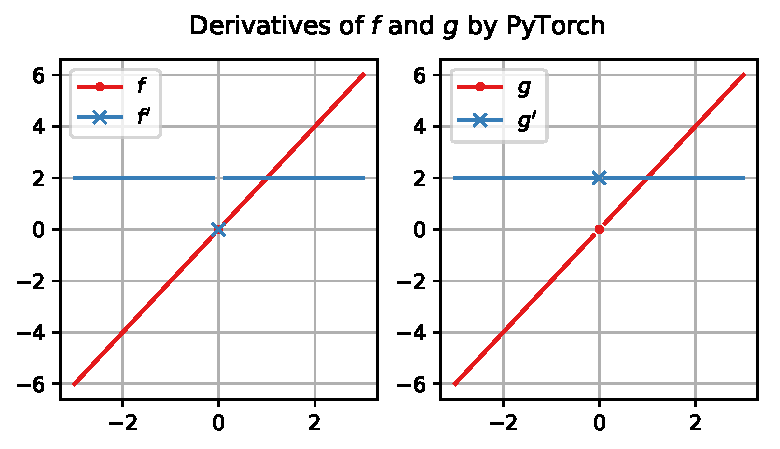
\includegraphics{problem4/problem4_differentiable.pdf}
  \caption{$f$ and $g$ from Listing \ref{lst:fg_diff} plotted along with
    their PyTorch-computed derivatives.}
  \label{fig:problem4_differentiable}
\end{figure}

\section*{Problem 5: Elementary properties of $l_2$ regularized logisitic regression}

\subsection*{The binary case}

Consider minimizing
\begin{equation}
  J(\mathbf{w}) = -l\left(\mathbf{w},\mathcal{D}_\mathrm{train}\right) + \lambda\left\lVert\mathbf{w}\right\rVert_2^2,
\end{equation}
where
\begin{equation}
  l\left(\mathbf{w},\mathcal{D}\right) = \sum_j \log \mathbf{P}\left(
    y^j \mid \mathbf{x}^j, \mathbf{w}
  \right)
\end{equation}
is the log-likelihood on the data set $\mathcal{D}$ for
$y^j \in \{ \pm 1 \}$

State if the following are true or false. Briefly explain your reasoning.

\begin{enumerate}
\item With $\lambda > 0$ and the features $x^j_k$ linearly separable,
  $J\left(\mathbf{w}\right)$ has multiple locally optimal solution.
  \subsubsection*{Solution}
  
  \emph{False}. When the features are linearly separable, we can push loss
  unregularized loss arbitrarily close to $0$ but the the loss is
  still convex. The sum of two convex functions is convex, so there
  will be global optimum.
  
\item Let
  $\hat{\mathbf{w}} = \argmin_{\mathbf{w}} J\left(\mathbf{w}\right)$ be
    a global optimum. $\hat{\mathbf{w}}$ is typically sparse.
    
    \subsubsection*{Solution}
    \emph{False}. This may be true with $l_1$ regularization, but is not
    usually the case with $l_2$ regularization. If one considers the
    dual Lagrangian problem, $\hat{\mathbf{w}}$ will lie on some
    hypersphere at a point which will not generally have $0$ values.
  \item If the training data is linearly separable, then some weights
    $w_j$ might become infinite if $\lambda = 0$.
    \subsubsection*{Solution}

    \emph{True}. By making the weights larger and larger we can push the loss
    to be arbitrarily close to $0$ if $\lambda = 0.$
    
  \item $l\left(\hat{\mathbf{w}}, \mathcal{D}_\mathrm{train}\right)$
    always increases as we increase $\lambda$.
    \subsubsection*{Solution}

    \emph{True}. If one thinks in term of the Lagrangian dual problem
    increasing $\lambda$ is contraining the weights further away from
    the global optimum by restricting them to a smaller hypersphere.

  \item $l\left(\hat{\mathbf{w}}, \mathcal{D}_\mathrm{test}\right)$
    always increases as we increase $\lambda$.
    \subsubsection*{Solution}

    \emph{False}. While the training loss may increase, we could be
    overfitting. Thus, sometimes increasing $\lambda$ may decrease
    test loss.    
\end{enumerate}

\subsection*{Multi-class Logistic Regression}

In multi-class logistic regression, suppose
$Y \in \left\{y_1,\ldots,y_R\right\}$. A simplified version (with no
bias term) is as follows. When $k < R$ the posterior probability is given by:
\begin{equation}
  P\left( Y = y_k \mid X\right) =
  \frac{\exp\left(\left\langle w_k, X\right\rangle\right)}
  {1 + \sum_{j=1}^{R-1}\exp\left(\left\langle w_j, X\right\rangle\right)}.
  \label{eqn:multiclass_log_reg}
\end{equation}

For $k = R$, the posterior is
\begin{equation}
  P\left( Y = y_R \mid X\right) =
  \frac{1}
  {1 + \sum_{j=1}^{R-1}\exp\left(\left\langle w_j, X\right\rangle\right)}.
\end{equation}

To simplify notation, we can define $w_R = \mathbf{0}$ as a vector of
all $0$s. This gives us Equation \ref{eqn:multiclass_log_reg} for all
$k$.

\begin{enumerate}
\item How many parameters do we need to estimate? What are these
  parameters?

  \subsubsection*{Solution}

  Assume the data is $D$-dimensional. Our parameters are the weights
  $w_k$ each which is a $D$-dimensional vector. There are
  $\boxed{(R - 1)D}$ parameters to estimate.
\item Given $N$ training samples
  $\left\{\left(x^1, y^1\right),\left(x^2,
      y^2\right),\ldots,\left(x^N, y^N\right)\right\}$, write down
  explicitly the log-likelihood function and simplify it as much as
  you can:
  \begin{equation}
    L\left(w_1,\ldots,w_{R-1}\right) = \sum_{j=1}^N \log\left(
      P\left(y^j \mid ^j,w\right)
    \right).
  \end{equation}
    
  \subsubsection*{Solution}
\item 
\item 
\end{enumerate}

\end{document}
% Local Variables:
% TeX-command-extra-options: "-shell-escape"
% End: